\chapter{Tracking, Spin, and Transfer Matrix Calculation Methods}
\label{c:methods}

\index{element!class}\index{tracking_method}
\index{mat6_calc_method}\index{spin_tracking_method}
\bmad allows for a number of methods that can be use to ``track'' a particle through a lattice
element. Here ``track'' can mean one of three things:
\begin{example}
  1) Calculate a particle's phase space coordinates at the exit 
     end of the element given the coordinates at the entrance end.
  2) Calculate the linear transfer map (Jacobian) through an element
     about a given reference orbit.
  3) Calculate the a particle's spin orientation at the exit end 
     of the element given the coordinates at the beginning.
\end{example}
The different tracking methods that are available have different advantages and disadvantages in
terms of speed, symplecticity, etc.  What tracking method is used, is selected on an
element--by--element basis using the attributes:
\begin{example}
  tracking_method      = <Switch>   ! phase space tracking method.
  mat6_calc_method     = <Switch>   ! 6x6 transfer matrix calculation.
  spin_tracking_method = <Switch>   ! Spin tracking method.
\end{example}
Example:
\begin{example}
  q2: quadrupole, tracking_method = symp_lie_ptc
  q2[tracking_method] = symp_lie_ptc
  quadrupole::*[tracking_method] = symp_lie_ptc
\end{example}
The first two lines of this example have exactly the same effect in terms of setting the
\vn{tracking_method}. The third line shows how to set the \vn{tracking_method} for an entire class
of elements.

These switches are discussed in more detail in the following sections.

%----------------------------------------------------------------------------
\section{Particle Tracking Methods}
\label{s:tkm}
\index{tracking methods|hyperbf}

The \vn{tracking_method} attribute of an element sets the algorithm that is used for single particle
tracking through that element.  Table~\ref{t:track.methods} gives which methods are available for
each type of element. Note: Table~\ref{t:track.methods} pertains to charged-particle tracking only.
When tracking photons, only \vn{bmad_standard} and \vn{custom} tracking method are available.

A note on terminology: Adaptive step size control used with the \vn{Runge_Kutta} integrator means
that instead of taking fixed step sizes the integrator chooses the proper step size so that the
error in the tracking is below the maximum allowable error set by \vn{rel_tol_adaptive_tracking} and
\vn{abs_tol_adaptive_tracking} tolerances. The advantage of step size control is that the integrator
uses a smaller step size when needed (the fields are rapidly varying), but makes larger steps when
it can. The disadvantage is that a step is more computationally intensive since the error in a step
is estimated by repeating a step using two mini steps. Except for testing purposes, it is
recommended that adaptive stepping be used over fixed step tracking since experience has shown that
adaptive stepping is almost always faster.  It is also recommended that \vn{runge_kutta} be used
over \vn{time_runge_kutta} since \vn{runge_kutta} does not have the overhead of switching between
time-coordinates and z-coordinates. The exceptions are cases where \vn{time_runge_kutta} must be
used like with an \vn{e_gun} where the particles start with zero momentum and in cases where
particles may reverse their longitudinal direction (EG: dark current electrons).

\begin{figure}[tb]
  \centering
  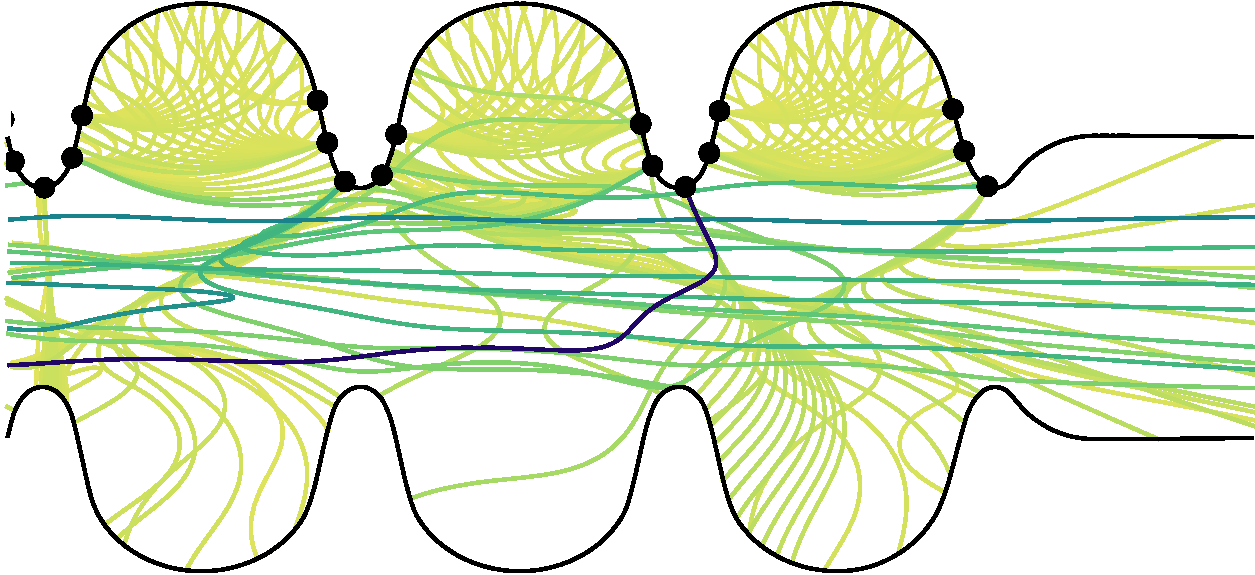
\includegraphics[width=4in]{dark-current.pdf}
  \caption[Dark current tracking.]{
Dark current tracking. Example of where a time based tracker (\vn{time_runge_kutta}) is useful for
simulating particles that can reverse their longitudinal velocity. Here the tracks drawn are from a
simulation of ``dark current'' electrons generated at the walls of an RF cavity due to the large
electromagnetic fields.  }
  \label{f:dark.current}
\end{figure}

\begin{description}

\index{bmad_standard!tracking_method}
\item[\vn{Bmad_Standard}]
Uses formulas for tracking. The formulas generally use the paraxial approximation. The emphasis here
is on speed. It is important to note that field maps (\sref{s:fieldmap}) are {\em ignored} by
\vn{bmad_standard} tracking. The tracking is non-symplectic but the non-symplectic errors tend to
be small so that \vn{bmad_standard} can be used in the vast majority of cases (\sref{s:non.symp}).

\index{custom!tracking_method}
\item[\vn{Custom}]
This method will call a routine \vn{track1_custom} which must be supplied by the programmer
implementing the custom tracking. The default \vn{track1_custom} supplied with the \bmad release
will print an error message and stop the program if it is called which probably indicates a program
linking problem. See \vn{s:custom.ele} for more details.

\index{fixed_step_runge_kutta!tracking_method}
\item[\vn{fixed_step_runge_kutta}]
The \vn{fixed_step_runge_kutta} method is similar to \vn{runge_kutta} tracking except that
\vn{fixed_step_runge_kutta} does not use adaptive step size control but instead takes steps of fixed
size using the setting of \vn{ds_step} or \vn{num_steps} for the element being tracked through
(\sref{s:integ}).  Generally, using adaptive step control will be much more efficient so it is
recommended that \vn{fixed_step_runge_kutta} {\em not} be used unless there is a compelling reason
not to. This method is non-symplectic (\sref{s:non.symp}).

\index{fixed_step_time_runge_kutta!tracking_method}
\item[\vn{fixed_step_time_runge_kutta}]
The \vn{fixed_step_time_runge_kutta} method is similar to \vn{time_runge_kutta} tracking except that
\vn{fixed_step_time_runge_kutta} does not use adaptive step size control but instead takes steps of
fixed size using the setting of \vn{ds_step} or \vn{num_steps} for the element being tracked through
(\sref{s:integ}).  Generally, using adaptive step control will be much more efficient so it is
recommended that \vn{fixed_step_time_runge_kutta} {\em not} be used unless there is a compelling
reason not to. This method is non-symplectic (\sref{s:non.symp}).

\index{linear!tracking_method}
\item[\vn{Linear}]
The \vn{linear} method just tracks particles using the 0th order vector with the 1st order 6x6
transfer matrix of an element. Depending upon how the transfer matrix was generated this may or may
not be symplectic. Since there would be a circular dependency to have the orbital tracking dependent
upon the transfer matrix and the transfer matrix dependent upon the determination of the reference
orbit, the calculation of the transfer matrix when the \vn{tracking_method} is set to \vn{linear}
will always use the zero orbit as the reference orbit.

Additionally, a \vn{linear} tracking method may not be used with \vn{mat6_calc_method} set to
\vn{tracking} since this would also give a circular dependency. Note: setting the
\vn{tracking_method} to \vn{linear} does not affect PTC calculations (\sref{s:ptc.intro}). In
particular, Taylor maps will not be affected.

\index{MAD!tracking_method}
\item[\vn{MAD}]
This uses the MAD 2nd order transfer map. This method is not able to handle element misalignments or
kicks, and becomes inaccurate as the particle energy deviates from the reference energy. MAD
tracking should only be used for testing purposes. Note: Thanks to CERN and Frank Schmidt for
permission to use the MAD tracking code within \bmad.

\index{runge_kutta!tracking_method}
\item[\vn{runge_kutta}]
This uses a 4\Th order Runge Kutta integration algorithm with adaptive step size control.  This is
essentially the Cash-Karp formulation. This method will be slow compared to non-Runge-Kutta methods
so only use this if it is not possible to use something like \vn{bmad_standard}.  This method is
accurate but non-symplectic (\sref{s:non.symp}). \vn{Warning:} When using \vn{custom} fields, if the
fields do not obey Maxwell's equation, there is the possibility of the \vn{runge_kutta} tracking
halting mid-way through an element. See section~\sref{s:integ} for more details.

\index{symp_lie_Bmad!tracking_method}
\item[\vn{Symp_Lie_Bmad}]
Symplectic tracking using a Hamiltonian with Lie operation techniques.  This is similar to
\vn{Symp_Lie_PTC} (see below) except this uses a \bmad routine. By bypassing some of the generality
inherent in PTC (\sref{s:ptc.intro}), \vn{Symp_Lie_Bmad} achieves about a factor of 10 improvement
in speed over \vn{Symp_Lie_PTC}.

\index{symp_lie_ptc!tracking_method}
\item[\vn{Symp_Lie_PTC}]
Symplectic tracking using a Hamiltonian with Lie operator techniques.  This uses \'Etienne Forest's
PTC (\sref{s:ptc.intro}) software for the calculation. This method is symplectic but can be
slow. Exceptions: The tracking is not symplectic when tracking through and element with an
associated electric field and when tracking through a \vn{taylor} element.

\index{taylor!tracking_method}
\item[\vn{Taylor}]
The tracking uses a Taylor map. The map is either explicitly given in the lattice file, that is, the
element must be of type \vn{taylor} (\sref{s:taylor}), or the Taylor map is generated from the PTC
(\sref{s:ptc.intro}) package. Generating the map may take time but once you have it it should be
very fast. One possible problem with using a Taylor map is that you have to worry about the accuracy
if you do tracking at points that are far from the expansion point about which the map was
made. This method is non-symplectic away from the expansion point. Whether the Taylor map is
generated taking into account the offset an element has is governed by the
\vn{taylor_map_includes_offsets} attribute (\sref{s:mapoff}).

The order of a Taylor map is set by the \vn{parameter[taylor_order]}
parameter (\sref{s:param}).

\index{time_runge_kutta!tracking_method}
\item[\vn{Time_Runge_Kutta}]
This method uses time as the independent variable instead of the longitudinal $z$ position. The
advantage of this method is that it can handle particles which reverse direction longitudinally.
One use for this method is ``dark current'' tracking where, as illustrated in \fig{f:dark.current},
low energy particles generated at the vacuum chamber walls can be found traveling in all
directions. Notice that \vn{time_runge_kutta} is different from using \vn{absolute time tracking} as
explained in \sref{s:rf.time}. This method is non-symplectic (\sref{s:non.symp}).

\end{description}

%----------------------------------------------------------------------------

\index{ab_multipole}\index{beambeam}\index{custom}
\index{drift}\index{ecollimator}\index{elseparator}\index{hkicker}
\index{instrument}\index{kicker}\index{lcavity}\index{marker}
\index{match}\index{monitor}\index{multipole}\index{octupole}
\index{patch}\index{quadrupole}\index{rbend}\index{rcollimator}\index{rf_bend}
\index{rfcavity}\index{sbend}\index{sextupole}\index{solenoid}
\index{sol_quad}\index{taylor}\index{vkicker}\index{wiggler}\index{capillary}
\index{element!table of class types}
\begin{table}[pht]
\centering {
\begin{tabular}{lccccccccc}  % \toprule
\rule{0pt}{80pt} 
{\em Element Class} &
\begin{sideways}\vn{Bmad_Standard}\end{sideways} &
\begin{sideways}\vn{Custom}\end{sideways} &
\begin{sideways}\vn{Linear}\end{sideways} &
\begin{sideways}\vn{MAD}\end{sideways} &
\begin{sideways}\vn{Runge_Kutta$^a$}\end{sideways} &
\begin{sideways}\vn{Symp_Lie_Bmad}\end{sideways} &
\begin{sideways}\vn{Symp_Lie_PTC}\end{sideways} &
\begin{sideways}\vn{Taylor}\end{sideways} &
\begin{sideways}\vn{Time_Runge_Kutta$^a$}\end{sideways}
\\ \midrule
%                                     BS   C   L   M   RK    SLB   SLP    T   TRK
  \vn{ab_multipole and multipole}    & D & X & X &   &     &     &  X  &  X  &    \\  
  \vn{ac_kicker}                     & D & X & X &   &  X  &     &     &     & X  \\  
  \vn{beambeam}                      & D & X & X &   &     &     &     &     &    \\  
  \vn{bends: rbend and sbend}        & D & X & X & X &     &     &  X  &  X  &    \\ 
  \vn{converter}                     & D & X &   &   &     &     &     &     &    \\  
  \vn{crab_cavity}                   & D & X & X &   &     &     &     &     &    \\  
  \vn{custom}                        &   & D & X &   &  X  &     &     &     & X  \\  
  \vn{drift}                         & D & X & X & X &  X  &     &  X  &  X  & X  \\  
  \vn{e_gun}                         &   & X &   &   &X$^b$&     &     &     & D  \\  
  \vn{ecollimator and rcollimator}   & D & X & X &   &  X  &     &  X  &  X  & X  \\  
  \vn{elseparator}                   & D & X & X & X &  X  &     &  X  &  X  & X  \\  
  \vn{em_field}                      &   & X &   &   &  D  &     &  X  &  X  & X  \\  
  \vn{fiducial}                      & D & X &   &   &     &     &  X  &     &    \\  
  \vn{floor_shift}                   & D & X &   &   &     &     &  X  &     &    \\  
  \vn{fork}                          & D & X & X &   &     &     &     &     &    \\
  \vn{gkicker}                       & D & X & X &   &     &     &  X  &  X  &    \\
  \vn{hkicker}                       & D & X & X &   &  X  &     &  X  &  X  & X  \\  
  \vn{instrument, monitor, and pipe} & D & X & X &   &  X  &     &  X  &  X  & X  \\  
  \vn{kicker}                        & D & X & X &   &  X  &     &  X  &  X  & X  \\  
  \vn{lcavity and rfcavity}          & D & X & X &   &  X  &     &  X  &  X  & X  \\  
  \vn{marker}                        & D & X & X &   &     &     &  X  &  X  &    \\  
  \vn{match}                         & D & X &   &   &     &     &     &  X  &    \\ 
  \vn{octupole}                      & D & X & X &   &  X  &     &  X  &  X  & X  \\ 
  \vn{patch}                         & D & X &   &   &X$^c$&     &  X  &  X  &    \\ 
  \vn{photonic elements}             & D & X &   &   &     &     &     &     &    \\
  \vn{quadrupole}                    & D & X & X & X &  X  &  X  &  X  &  X  & X  \\ 
  \vn{rf_bend}                       &   & X & X &   &  X  &     &     &     & X  \\
  \vn{sad_mult}                      & D & X & X &   &     &     &  X  &  X  &    \\
  \vn{sextupole}                     & D & X & X & X &  X  &     &  X  &  X  & X  \\ 
  \vn{solenoid}                      & D & X & X & X &  X  &  X  &  X  &  X  & X  \\ 
  \vn{sol_quad}                      & D & X & X &   &  X  &  X  &  X  &  X  & X  \\ 
  \vn{taylor}                        &   & X & X &   &     &     &  X  &  D  &    \\ 
  \vn{vkicker}                       & D & X & X &   &  X  &     &  X  &  X  & X  \\ 
  \vn{wiggler} (map type)            &   & X & X &   &  X  &  X  &  X  &  X  & X  \\
  \vn{wiggler} (periodic type)       & D & X & X &   &X$^d$&X$^d$&X$^d$&D$^d$&    \\ 
  \bottomrule
  \multicolumn{10}{l}{$^a$Includes fixed step versions.}                    \\
  \multicolumn{10}{l}{$^b$Only if the beginning energy is non-zero.}        \\
  \multicolumn{10}{l}{$^c$Only available for non-reflection patch elements.}\\
  \multicolumn{10}{l}{$^d$See \sref{s:wiggler.periodic} for more details.}  \\
\end{tabular}
}
\caption[Table of available tracking_method switches.] { 
Table of valid tracking_method switches. ``D'' denotes the
default method. ``X'' denotes a valid method. Photonic
elements are elements in Table~\ref{t:photon.classes} that cannot be used for
charged particle tracking (Table~\ref{t:particle.classes}).}

\label{t:track.methods}
\end{table}

\vfill \break

%----------------------------------------------------------------------------
\section{Linear Transfer Map (Mat6) Calculation Methods}
\label{s:xfer}
\index{mat6_calc_method|hyperbf}

The \vn{mat6_calc_method} attribute sets how the 6x6 Jacobian transfer matrix for a given element is
computed. Table~\ref{t:mat6.methods} gives which methods are available for each type of element.
Note: Table~\ref{t:mat6.methods} is for charged-particle tracking only. When tracking photons,
transfer matrices (which are not very useful) are not computed.

If an element's \vn{static_linear_map} parameter is set to \vn{True} (the default is \vn{False}),
this prevents the linear map, which consists of the transfer matrix and the zeroth order part of the
map, from being recomputed. For example, if somewhere in a lattice a steering is changed, this will
shift the reference orbit and the linear transfer map in elements where the reference orbit changes
will, in general, vary. However, having \vn{static_linear_map} set to \vn{True} will prevent this
variation.

\index{sympliectify}
\index{taylor_map_includes_offsets}
In addition to the \vn{mat6_calc_method} switch, two element attributes that can affect the way the
transfer matrix is calculated are \vn{symplectify} and \vn{taylor_map_includes_offsets}. These are
discussed in sections \sref{s:symp} and \sref{s:mapoff} respectively.

For methods that do not necessarily produce a symplectic matrix the \vn{symplectify} attribute of an
element can be set to \vn{True} to solve the problem. See \sref{s:symp.method}.

Symplectic integration is like ordinary integration of a function f(x) but what is integrated here
is a Taylor map. Truncating the map to 0\Th order gives the particle trajectory and truncating to
1\St\ order gives the transfer matrix (Jacobian).  The order at which a Taylor series is truncated
at is set by \vn{taylor_order} (see \sref{s:param}. Like ordinary integration there are various
formulas that one can use to do symplectic integration.

\begin{description}

\index{auto!mat6_calc_method}
\item[\vn{Auto}]
With \vn{auto} the \vn{mat6_calc_method} appropriate for the element's setting of
\vn{tracking_method} is used. The correspondence is:
\begin{table}[pth]
\centering {
\begin{tabular}{ll} \toprule
Element's \vn{tracking_method} & \vn{Mat6_calc_method} used\\
\midrule
\vn
  \vn{bmad_standard}         & \vn{bmad_standard} \\
  \vn{linear}                & \vn{bmad_standard} \\
  \vn{custom}                & \vn{custom} \\
  \vn{mad}                   & \vn{mad} \\
  \vn{symp_lie_bmad}         & \vn{symp_lie_bmad} \\
  \vn{symp_lie_ptc}          & \vn{symp_lie_ptc} \\
  \vn{taylor}                & \vn{taylor} \\
  All \vn{Runge-Kutta} types & \vn{tracking} \\
\bottomrule
\end{tabular}
}
\caption[Actual \vn{mat6_calc_method} used with \vn{auto} setting.]{Actual \vn{mat6_calc_method} used when
when the \vn{mat6_calc_method} is set to \vn{auto}.}
\end{table}

\index{bmad_standard!mat6_calc_method}
\item[\vn{Bmad_Standard}]
Uses formulas for the calculation. The formulas generally use the paraxial approximation. The
emphasis here is on speed.

\index{custom!mat6_calc_method}
\item[\vn{Custom}]
This method will call a routine \vn{make_mat6_custom} which must be supplied by the programmer
implementing the custom transfer matrix calculation. The default \vn{make_mat6_custom} supplied with
the \bmad release will print an error message and stop the program if it is called which probably
indicates a program linking problem.  See \vn{s:custom.ele} for more details.

\index{MAD!mat6_calc_method}
\item[\vn{MAD}]
This uses the MAD 2nd transfer map. This method is not able to handle element misalignments or
kicks, and becomes inaccurate as the particle energy deviates from the reference energy. MAD
tracking is generally only used for testing purposes. Thanks must be given to CERN and Frank Schmidt
for permission to use the MAD tracking code within \bmad.

\index{symp_lie_bmad!mat6_calc_method}
\item[\vn{Symp_Lie_Bmad}]
A symplectic calculation using a Hamiltonian with Lie operator techniques.  This is similar to
\vn{Symp_Lie_PTC} (see below) except this uses a \bmad routine. By bypassing some of the generality
inherent in PTC, \vn{Symp_Lie_Bmad} achieves about a factor of 10 improvement in speed over
\vn{Symp_Lie_PTC}. However, \vn{Symp_Lie_Bmad} cannot generate maps above first order.

\index{symp_lie_ptc!mat6_calc_method}
\item[\vn{Symp_Lie_PTC}]
Symplectic integration using a Hamiltonian and Lie operators.  This uses the PTC
(\sref{s:ptc.intro}) software for the calculation.  This method is symplectic but can be
slow. Exceptions: The tracking is not symplectic when tracking through and element with an
associated electric field and when tracking through a \vn{taylor} element.

\index{taylor!mat6_calc_method}
\item[\vn{Taylor}]
This uses a Taylor map generated from \'Etienne's PTC package. Generating the map may take time but
once you have it it should be very fast. One possible problem with using a Taylor map is that you
have to worry about the accuracy if you do a calculation at points that are far from the expansion
point about which the map was made. This method is non-symplectic away from the expansion
point. Whether the Taylor map is generated taking into account the offset an element has is governed
by the \vn{taylor_map_includes_offsets} attribute (\sref{s:mapoff}). \vn{bmad_standard} and
\vn{taylor} tracking methods are identical. Note: Taylor maps for \vn{match}, and \vn{patch}
elements are limited to first order.

The order of a Taylor map is set by the \vn{parameter[taylor_order]}
parameter (\sref{s:param}).

\index{tracking!mat6_calc_method}
\item[\vn{Tracking}]
This uses the tracking method set by \vn{tracking_method} to track 6 particles around the central
orbit. This method is susceptible to inaccuracies caused by nonlinearities. Furthermore this method
is almost surely slow. While non--symplectic, the advantage of this method is that it is directly
related to any tracking results. Note: a \vn{linear} tracking method may not be used with
\vn{mat6_calc_method} set to \vn{tracking} since this would give a circular dependency. The two
parameters that affect this calculation are \vn{bmad_com%d_orb(6)} (\sref{s:bmad.common}) which
sets the six deltas used for displacing the initial particle coordinates from the reference orbit.

\end{description}

\index{ab_multipole}\index{beambeam}\index{custom}
\index{drift}\index{ecollimator}\index{elseparator}\index{hkicker}
\index{instrument}\index{kicker}\index{lcavity}\index{marker}
\index{match}\index{monitor}\index{multipole}\index{octupole}
\index{patch}\index{quadrupole}\index{rbend}\index{rcollimator}
\index{rfcavity}\index{sbend}\index{sextupole}\index{solenoid}
\index{sol_quad}\index{taylor}\index{vkicker}\index{wiggler}
\index{crystal}\index{capillary}\index{rf_bend}
\begin{table}[pth]
\centering {
\begin{tabular}{lcccccccc} \toprule
\rule{0pt}{80pt} &
\begin{sideways}\vn{Bmad_Standard}\end{sideways} &
\begin{sideways}\vn{Custom}\end{sideways} &
\begin{sideways}\vn{MAD}\end{sideways} &
\begin{sideways}\vn{Static}\end{sideways} &
\begin{sideways}\vn{Symp_Lie_Bmad}\end{sideways} &
\begin{sideways}\vn{Symp_Lie_PTC}\end{sideways} &
\begin{sideways}\vn{Taylor}\end{sideways} &
\begin{sideways}\vn{Tracking}\end{sideways}
\\ \midrule
%                                     BS   C   M  Stat SLB   SLP   Tlr  Trk
  \vn{ab_multipole and multipole}    & D & X &   & X &     &  X  &  X  & X \\  
  \vn{ac_kicker}                     &   & X &   & X &     &  X  &  X  & D \\  
  \vn{beambeam}                      & D & X &   & X &     &     &     & X \\  
  \vn{bends: rbend and sbend}        & D & X & X & X &     &  X  &  X  & X \\ 
  \vn{converter}                     & D & X &   &   &     &     &     &   \\  
  \vn{crab_cavity}                   &   & X &   & X &     &     &     & D \\  
  \vn{custom}                        &   & D &   & X &     &     &     & X \\  
  \vn{drift}                         & D & X & X & X &     &  X  &  X  & X \\  
  \vn{e_gun}                         &   & X &   & X &     &     &     & D \\  
  \vn{ecollimator and rcollimator}   & D & X &   & X &     &  X  &  X  & X \\  
  \vn{elseparator}                   & D & X & X & X &     &  X  &  X  & X \\  
  \vn{em_field}                      &   & X &   & X &     &  X  &  X  & D \\  
  \vn{fiducial}                      & D & X &   & X &     &  X  &     & X \\  
  \vn{floor_shift}                   & D & X &   & X &     &  X  &     & X \\  
  \vn{hkicker}                       & D & X &   & X &     &  X  &  X  & X \\  
  \vn{instrument, monitor, and pipe} & D & X &   & X &     &  X  &  X  & X \\  
  \vn{kicker}                        & D & X &   & X &     &  X  &  X  & X \\  
  \vn{lcavity and rfcavity}          & D & X &   & X &     &  X  &  X  & X \\  
  \vn{marker}                        & D & X &   & X &     &  X  &  X  & X \\  
  \vn{match}                         & D & X &   & X &     &     &     & X \\  
  \vn{octupole}                      & D & X &   & X &     &  X  &  X  & X \\ 
  \vn{patch}                         & D & X &   & X &     &  X  &  X  & X \\ 
  \vn{quadrupole}                    & D & X & X & X &  X  &  X  &  X  & X \\ 
  \vn{rf_bend}                       & D & X &   & X &     &     &     & X \\
  \vn{sad_mult}                      & D & X &   & X &     &  X  &  X  & X \\ 
  \vn{sextupole}                     & D & X & X & X &     &  X  &  X  & X \\ 
  \vn{solenoid}                      & D & X & X & X &  X  &  X  &  X  & X \\ 
  \vn{sol_quad}                      & D & X & X & X &  X  &  X  &  X  & X \\ 
  \vn{taylor}                        &   & X &   & X &     &  X  &  D  &   \\ 
  \vn{vkicker}                       & D & X &   & X &     &  X  &  X  & X \\ 
  \vn{wiggler} (map type)            & D & X &   & X &X$^a$&X$^a$&X$^a$& X \\ 
  \vn{wiggler} (periodic type)       &   & X &   & X &X$^a$&X$^a$&D$^a$& X \\ \bottomrule
  \multicolumn{9}{l}{$^a$See \sref{s:wiggler.periodic} for more details} \\
\end{tabular}
} 
\caption[Table of available mat6_calc_method switches.]  {Table of
available mat6_calc_method switches. When tracking photons, transfer
matrices are not computed.  ``D'' denotes the default method. ``X'' denotes an available method.}

\label{t:mat6.methods}
\end{table}

\vfill \break

%----------------------------------------------------------------------------
\section{Spin Tracking Methods}
\label{s:spin.methods}
\index{spin tracking!methods}
\index{spin_tracking_method}

The \vn{spin_tracking_method} attribute of an elements sets the algorithm that is used for tracking
a particle's spin (\sref{s:spin.dyn}) through that element.  Table~\ref{t:spin.methods} gives which
methods are available for each type of element. Note: This table is only for charged-particle tracking
since photons do not have spin.

Possible \vn{spin_tracking_method} settings are:
\begin{description}
%
\index{custom!spin_tracking_method}
\item[\vn{Custom}] \Newline
This method will call a routine \vn{track1_spin_custom} which must be supplied by the programmer
implementing the custom spin tracking calculation. See \vn{s:custom.ele} for more details.
%
\item[\vn{Magnus}] \Newline
This method uses a second-order Magnus expansion of the T-BMT equation to track spins (\sref{s:magnus}).
It is fast and in most cases closely matches numerical integration.
%
\item[\vn{Off}] \Newline
No spin tracking is done and the spin at the end of the element is the same as at the beginning.
%
\item[\vn{Sprint}] \Newline
The \vn{sprint} algorithm (\sref{s:sprint.std}) uses first order transfer spin maps to track the
spin through lattice elements. This method is very fast at the cost of accuracy for particles away
from the zero orbit. The algorithm is also limited in what elements it can handle and it ignores
higher order multipoles that may be present.
%
\index{symp_lie_ptc!spin_tracking_method}
\item[\vn{Symp_Lie_PTC}] \Newline
Symplectic integration using a Hamiltonian and Lie operators.  This uses \'Etienne's PTC software
for the calculation.  This method is symplectic but can be slow.
%
\index{tracking!spin_tracking_method}
\item[\vn{Tracking}] \Newline
How spin is tracked here will depend also on the setting of \vn{tracking_method}. If
\vn{tracking_method} is set to \vn{runge_kutta} or \vn{time_runge_kutta} the spin will be tracked
along with the phase space particle coordinates using the local fields. For \vn{tracking_method} set
to \vn{symp_lie_ptc}, the spin tracking will use \vn{PTC}.  For all other \vn{tracking_method}s, the
spin will be tracked using the ``\vn{bmad_standard}'' spin tracking method which involves Romberg
integration of the spin rotation matrix.

The \vn{runge_kutta} and \vn{time_runge_kutta} spin tracking uses the same fourth order integrator
as is used for the orbital coordinates to track the spin rotation vector.
%
\item[\vn{Transverse_Kick}] \Newline
With a setting of \vn{transverse_kick}, it is assumed that the orbital transfer matrix is due solely
to transverse magnetic fields so that the integrated spin rotation (\Eqs{orpt}, \eq{pqlbp1}, and
\eq{pqlbp2}) can be related to the orbital transport via
\begin{equation}
  \int {\pmb\Omega}_{BMT} = \frac{1 + a \gamma}{1 + p_z} \, (-\Delta p_y, \Delta p_x, 0)
\end{equation}
where $\Delta p_x$ and $\Delta p_y$ are the change in $p_x$ and $p_y$.
Here the small angle approximation ($p_x, p_y \ll 1$) has been used.
\end{description}


%-----------------
Since speed may be an issue, \bmad has an global parameter called \vn{spin_tracking_on} which is
part of the \vn{bmad_com} instance (\sref{s:bmad.ptc.com}) that determines whether spin is tracked or
not. Note: There is also another \vn{bmad_com} parameter called \vn{spin_baier_katkov_flipping_on}
which can influence spin tracking.

\index{spin_fringe_on}
The \vn{spin_fringe_on} element attribute (\sref{s:fringe.at}) can be used to toggle whether the
fringe fields of an element affect the spin.

Example:
\begin{example}
  q: quadrupole, spin_tracking_method = symp_lie_ptc
\end{example}


\index{ab_multipole}\index{beambeam}\index{custom}
\index{drift}\index{ecollimator}\index{elseparator}\index{hkicker}
\index{instrument}\index{kicker}\index{lcavity}\index{marker}
\index{match}\index{monitor}\index{multipole}\index{octupole}
\index{patch}\index{quadrupole}\index{rbend}\index{rcollimator}
\index{rfcavity}\index{sbend}\index{sextupole}\index{solenoid}
\index{sol_quad}\index{taylor}\index{vkicker}\index{wiggler}
\index{crystal}\index{capillary}
\begin{table}[pth]
\centering {
\begin{tabular}{lccccccc} \toprule
\rule{0pt}{80pt} &
\begin{sideways}\vn{Off}\end{sideways} &
\begin{sideways}\vn{Custom}\end{sideways} &
\begin{sideways}\vn{Magnus}\end{sideways} &
\begin{sideways}\vn{Sprint}\end{sideways} &
\begin{sideways}\vn{Symp_Lie_PTC}\end{sideways} &
\begin{sideways}\vn{Tracking}\end{sideways}
\begin{sideways}\vn{Transverse_Kick}\end{sideways} &
\\ \midrule
%                                      O   C   M  Spt SLP Trk TK
  \vn{ab_multipole and multipole}    & X & X &   &   &   & D &   \\  
  \vn{ac_kicker}                     & X & X &   &   &   & D &   \\  
  \vn{beambeam}                      & X & X &   &   &   & D &   \\  
  \vn{bends: rbend and sbend}        & X & X & X  & X & X & D &   \\ 
  \vn{converter}                     & X & X &   &   &   & D &   \\  
  \vn{crab_cavity}                   & X & X &   &   &   & D &   \\  
  \vn{custom}                        & X & D &   &   &   & X &   \\  
  \vn{drift}                         & X & X & X & X & X & D &   \\  
  \vn{e_gun}                         & X & X &   &   &   & D &   \\  
  \vn{ecollimator and rcollimator}   & X & X &   & X & X & D &   \\  
  \vn{elseparator}                   & X & X &   &   & X & D &   \\  
  \vn{em_field}                      & X & X &   &   &   & D &   \\  
  \vn{fiducial}                      & X & X &   &   & X & D &   \\  
  \vn{floor_shift}                   & X & X &   &   & X & D &   \\  
  \vn{hkicker}                       & X & X & X & X & X & D &   \\  
  \vn{instrument, monitor and pipe}  & X & X & X  & X & X & D &   \\  
  \vn{kicker}                        & X & X & X & X & X & D &   \\  
  \vn{lcavity and rfcavity}          & X & X & X &   & X & D &   \\  
  \vn{marker}                        & X & X & X &   & X & D &   \\  
  \vn{match}                         & D &   &   &   &   &   & X \\  
  \vn{octupole}                      & X & X &   & X & X & D &   \\ 
  \vn{patch}                         & X & X &   &   & X & D &   \\ 
  \vn{quadrupole}                    & X & X & X & X & X & D &   \\ 
  \vn{sad_mult}                      & X & X &   &   &   & D &   \\  
  \vn{sextupole}                     & X & X & X & X & X & D &   \\ 
  \vn{solenoid}                      & X & X & X & X & X & D &   \\ 
  \vn{sol_quad}                      & X & X &   &   & X & D & X \\ 
  \vn{taylor}                        & X &   &   &   &   & D &   \\ 
  \vn{vkicker}                       & X & X & X & X & X & D &   \\ 
  \vn{wiggler}                       & X & X &   &   & X & D &   \\ 
  \bottomrule
\end{tabular}
}

\caption[Table of available spin_tracking_method switches.]{Table of
available \vn{spin_tracking_method}\ switches. ``D'' denotes the default method. 
``X'' denotes an available method. Note: Photon tracking does not involve spin.}

\label{t:spin.methods}
\end{table}

\vfill \break

%-----------------------------------------------------------------
\section{Integration Methods}
\label{s:integ}
\index{integration methods}

\index{symp_lie_bmad!and Taylor maps}
\index{symp_lie_ptc!and Taylor maps}
\index{taylor!and Taylor maps}
``Integration methods'' are tracking methods that involve integrating through an element's magnetic
and electric fields.  Integration methods are split into two classes: Those that can track Taylor
maps and those that simply track a particle's position.  The Taylor map methods are
\begin{example}
  symp_lie_bmad   ! Only to first order
  symp_lie_ptc    ! Uses PTC
  taylor          ! Uses PTC
\end{example}
See section \sref{s:taylor.phys} for more information on Taylor maps and symplectic integration. The
latter two methods involve using the PTC library (\sref{s:ptc.intro}).

The methods that do not involve Taylor maps are
\index{runge_kutta!and Taylor maps}
\begin{example}
  fixed_step_runge_kutta
  fixed_step_time_runge_kutta
  runge_kutta
  time_runge_kutta
\end{example}

\index{ds_step}\index{num_steps}\index{integrator_order}
\index{field_calc}\index{csr_method}\index{space_charge_method}
there are a number of element attributes that can affect the calculation. They are
\begin{example}
  ds_step             = <Real>     ! Integration step length (\sref{s:ds.step})
  num_steps           = <Integer>  ! Number of integration steps. (\sref{s:ds.step})
  integrator_order    = <Integer>  ! Integrator order (\sref{s:ptc.integ})
  field_calc          = <Switch>   ! How the field is calculated (\sref{s:field.calc})
\end{example}

Example:
\begin{example}
  q1: quadrupole, l = 0.6, tracking_method = bmad_standard, 
        mat6_calc_method = symp_lie_ptc, ds_step = 0.2, field_calc = custom
\end{example}

%-----------------------------------------------------------------
\section{CSR and Space Charge Methods}
\label{s:csr.sc.meth}
\index{csr and space charge methods}

When doing beam tracking through an element (\sref{c:multi.sim}), Coherent Synchrotron Radiation
(CSR) and Space Charge (SC) effects can be included by setting the appropriate method switches in
that element. These switches are:
\begin{example}
  csr_method          = <Switch>   ! Coherent Synchrotron Radiation 
  space_charge_method = <Switch>   ! Space charge method
\end{example}
Note: For CSR or SC effects to be included in tracking the \vn{bmad_com} logical
\vn{csr_and_space_charge_on} must be set to \vn{True} (\sref{s:bmad.common}).

The possible settings for \vn{csr_method} are
\begin{example}
  off             ! No CSR. Default.
  1_dim           ! One dimensional calculation (\sref{s:csr.1d}).
\end{example}
The \vn{1_dim} setting cannot be used when \vn{space_charge_method} is set to  \vn{cathode_fft_3d}.

The possible settings of \vn{space_charge_method} are
\begin{example}
  off             ! No SC. Default.
  slice           ! SC using slices (\sref{s:sc.slice}).
  fft_3d          ! SC using a 3D grid (\sref{s:sc.fft}).
  cathode_fft_3d  ! Same as fft_3d with cathode image charge included (\sref{s:sc.fft}).
\end{example}
The \vn{cathode_fft_3d} setting can only be used with \vn{csr_method} set to \vn{off}. Additionally,
the \vn{cathode_fft_3d} setting can only be used with the element \vn{tracking_method} set to
\vn{time_runge_kutta} or \vn{fixed_step_time_runge_kutta}.

Example:
\begin{example}
  q1: quadrupole, l = 0.6, csr_method = 1_dim, space_charge_method = slice, ...
\end{example}

Also see the \vn{space_charge_com} structure (\sref{s:sc.com}) which contains parameters used in
space charge and CSR calculations.

Note: There is also high energy space charge calculation that can be used with single particle
tracking and is discussed in \sref{s:he.space.charge}.

%-----------------------------------------------------------------
\subsection{ds_step and num_steps Parameters}
\label{s:ds.step}
\index{ds_step}\index{num_steps}

\index{taylor}\index{symp_lie_ptc}\index{symp_lie_bmad}
\index{runge_kutta}
One way to create a transfer map through an element is to divide the element up into slices and then
to propagate the transfer map slice by slice.  There are several ways to do this integration. The
\vn{runge_kutta} type methods integrate the equations of motion to give the 0\Th order Taylor map
which just represents a particle's orbit.  Symplectic integration\index{symplectic!integration}
using Lie algebraic techniques, on the other hand, can generate Taylor maps to any order. The
\vn{ds_step} attribute determines the slice thickness.  Alternatively, \vn{num_steps} attribute can
be used in place of \vn{ds_step} to specify the number of slices.  This is applicable to
\vn{symp_lie_bmad} and \vn{symp_lie_ptc} integration. Example:
\begin{example}
  q: quadrupole, l = 0.6, ds_step = 0.1  ! 10 cm step size.
  sbend::*[ds_step] = 0.2                ! Set the step_size for all sbend elements.
\end{example}

When tracking using maps or element-by-element with PTC there are a few points to keep in
mind. First is that \vn{PTC} tracks through a lattice element step by step. This is true for both
map creation and symplectic integration. This means that the setting of the element parameter
\vn{integrator_order} (\sref{s:ptc.integ})
or \vn{num_steps} (or \vn{ds_step}) for each element will affect the accuracy and speed of the
computations. Bmad tries to choose reasonable default settings for the integrator order and number
of steps however the calculation is not perfect. To make sure that the integrator order and number
of steps is set properly, vary both and choose values (which can be different for different
elements) such that the number of steps and integrator order is minimal (to minimize computation
time) while at the same time is large enough so that results do not change significantly if the
number of steps or is varied. Generally it is much better to use a large integrator order and a
small step size rather than vice versa with the proviso that for elements with a longitudinally
varying field (think wigglers or undulators), the step size must be small compared to the typical
longitudinal length scale over which the field is varying (this length scale is the pole period
length with with wigglers and undulators).

The default value for \vn{ds_step} for a given element is calculated based upon the element's field
strength. One should consider the default as more of a guesstimate.

\index{ds_step}
\index{runge_kutta}\index{time_runge_kutta}
\index{rel_tol_adaptive_tracking}\index{abs_tol_adaptive_tracking}
The \vn{runge_kutta} and \vn{time_runge_kutta} tracking uses adaptive step control independent of
the setting of the elements \vn{ds_step} parameter. These methods use three \vn{bmad_com} parameters
\sref{s:bmad.ptc.com}) namely:
\begin{example}
  bmad_com[rel_tol_adaptive_tracking]
  bmad_com[abs_to_adaptive_tracking]
  bmad_com[max_num_runge_kutta_step]
\end{example}
The estimated error of the integration is then bounded by
\begin{example}
  error < abs_tol + |orbit| * rel_tol
\end{example}
lowering the error bounds makes for greater accuracy (as long as round-off 
doesn't hurt) but for slower tracking. 

%-----------------------------------------------------------------
\subsection{Field_calc Parameter}
\label{s:field.calc}
\index{field_calc}

\index{runge_kutta}
The \vn{runge_kutta} type tracking methods all use as input the electric and magnetic fields of
an element. How the EM fields are calculated is determined by the \vn{field_calc} attribute for an
element.  For all lattice elements, except \vn{wigglers} and \vn{undulators}, possible values for
\vn{field_calc} are:
\begin{example}
  bmad_standard     ! This is the default except for custom elements
  custom            ! Default for custom elements.
  fieldmap
\end{example}
For \vn{wigglers} and \vn{undulators}, possible values for \vn{field_calc} are:
\begin{example}
  planar_model
  helical_model
  custom
  fieldmap
\end{example}
\index{custom}\index{runge_kutta}
For historical reasons, the default setting for \vn{field_calc} for \vn{wigglers} and
\vn{undulators} is \vn{planar_model} except if there is a field map present (\sref{s:fieldmap}) in
which case the default is \vn{fieldmap}.  Note that with \vn{bmad_standard} tracking, the setting of
\vn{field_calc} is ignored except in the case of \vn{wigglers} and \vn{undulators} where
\vn{field_calc} must be set to either \vn{planar_model} or \vn{helical_model}.

\vn{Custom} means that the field calculations are done outside of the \bmad software. A program
doing \vn{custom} field calculations will need the appropriate custom routine (\sref{s:custom.ele}).
Elements that set \vn{field_calc} to \vn{fieldmap} need to have a field map defined
(\sref{s:fieldmap}).

\vn{Warning:} When tracking a particle through a custom field using \vn{runge_kutta}, it is
important that the field obey Maxwell's equations. Fields that do not obey Maxwell's Equations may
cause the \vn{runge_kutta} adaptive step size control algorithm to take smaller and smaller steps
until the step size becomes so small the tracking will stop. What happens is that the step size
control algorithm takes a step and then takes two half steps over the same region and from this
estimates the error in the calculation. If the error is larger than the allowed tolerance the
control algorithm shortens the step and tries again. A field that does not obey Maxwell's equations
can fool the control algorithm into thinking that the error is always larger than the allowed
tolerance for any finite step size. A typical situation is where the field has an unphysical step
across some boundary.

%-----------------------------------------------------------------
\subsection{PTC Integration}
\label{s:ptc.integ}
\index{PTC integration}

\index{integrator_order}
\index{ds_step}\index{symp_lie_bmad}
The \vn{integrator_order} element attribute is the order of the integration formula for
\vn{Symp_Lie_PTC} and is used for constructing Taylor maps. Possible values are
\begin{example}
  integrator_order = 2, 4, 6, or 8
\end{example}
Essentially, an integrator order of $n$ means that the error in an integration step scales as
$dz^{n+1}$ where $dz$ is the slice thickness. For a given number of steps a higher order will give
more accurate results but a higher order integrator will take more time per step. It turns out that
for wigglers, after adjusting \vn{ds_step} for a given accuracy, the order 2 integrator is the
fastest. This is not surprising given the highly nonlinear nature of a wiggler. Note that
\vn{symp_lie_bmad} always uses an order 2 integrator independent of the setting of
\vn{integrator_order}. The setting of \vn{8} is not implemented for all elements. If \vn{8} is set
for a given element type that does not support it, a value of \vn{6} will be used instead.

\index{exact_model}\index{exact_misalign}
When tracking uses the \vn{PTC} library (\sref{s:ptc.intro}), there are two global parameters that
can be set in the lattice file that affect the calculation. These are:
\begin{example}
  ptc_com[exact_model]    = <Logical>  ! "exact" tracking? Default: False
  ptc_com[exact_misalign] = <Logical>  ! "exactly" misalign elements? Default: True
\end{example}
The default for \vn{exact_model} is \vn{True} and the default for \vn{exact_misalign} is \vn{True}.

The \vn{exact_model} parameter sets whether PTC uses an ``exact'' model for
tracking. Essentially this means that the paraxial approximation (\sref{s:mag.hamiltonian}) is made
for \vn{exact_model} set to \vn{False} and is not made if set to \vn{True}. This can be
important, for example, for bend tracking when the bend radius is small.

In PTC, exact modeling can be set on an element-by-element basis. Currently \bmad does not support
specifying element-by-element setting of exact modeling. However, PTC does not have a non-exact
tracking option for elements that have an electric field. In this case, PTC tracking will always be
exact independent of the setting of \vn{exact_model}.  Additionally, for elements with an
electric field, tracking will not be symplectic.

The \vn{exact_misalign} parameter determines whether misalignments are handled exactly or
whether approximations are made that will speed up the calculation.

In addition to the above parameters, how the Hamiltonian is split when tracking with \vn{PTC} can be
set for individual elements using the \vn{ptc_integration_type} parameter. Possible settings of this
parameter are
\begin{example}
  drift_kick    ! See Eq. (125) of \cite{b:geo.int}
  matrix_kick   ! See Eq. (132) of \cite{b:geo.int}. Default
  ripken_kick   ! See Eq. (130) of \cite{b:geo.int}
\end{example}
Example:
\begin{example}
  q2: quad, l = 0.6, k1 = 0.34, ptc_integration_type = drift_kick
\end{example}
A discussion of the different types of integration schemes is given by Forest\cite{b:geo.int}. The
equation that shows the appropriate splitting of the Hamiltonian for each integration type is
referenced in the above list. The \vn{ripken_kick} type is for benchmarking with the \vn{SixTrack}
program and is not otherwise generally useful. The difference between \vn{drift_kick} and
\vn{matrix_kick} is that with \vn{drift_kick} the quadrupolar part of the magnetic multipole is is
included in the applied kick between drifts while in the \vn{matrix_kick} method the quadrupolar
component is used for the ``matrix'' tracking between kicks. With the \vn{matrix_kick} method the
tune of a machine tends to be insensitive to how many integration steps (set by \vn{ds_step} or
\vn{n_steps}) are used.

PTC does not implement \vn{matrix_kick} tracking for elements with an electric field. In this case,
the setting of \vn{ptc_integration_type} is ignored and tracking will be \vn{drift_kick}. Thus, if
an electric field is introduced into an element, more integration steps may be required to get the
correct tune.

%-----------------------------------------------------------------
\section{Symplectic Versus Non-Symplectic Tracking}
\label{s:non.symp}
\index{symplectify}

When selecting tracking methods for lattice elements, there are several factors to consider,
including symplecticity. Despite its emphasis in accelerator textbooks, symplecity (or the lack
therof) is typically only relevant for long-term tracking when there is minimal radiation emission
over many turns. That is, the potential problem with non-symplectic tracking is the buildup of
errors over many turns. Thus, computations that involve only tracking through the lattice from
beginning to end -- like calculating Twiss functions or tracking through a linac -- generally do not
benefit from symplectic tracking. More important in these cases is the speed of the calculation, 
which can be obtained with the cost of non-symplecticity.

The motion of particles that radiate is not symplectic. Thus, symplectic tracking for the
non-radiative part of the motion may not be needed if radiation is large enough. For example, for
simulations of the Cornell CESR ring with electron and positron beam energies of order 1~GeV to
10~GeV and with damping times on the order of 10,000 turns, the \vn{bmad_standard} tracking has
proved quite adequate. However in other cases with radiation, the symplectic error may cause an 
extra damping or anti-damping effect, giving equilibrium beam sizes that are an under/overestimate 
of the actual beam sizes. When opting for speed versus symplecticity in long term tracking over 
many turns, care should be taken to ensure that the effects of the non-symplecticity are minimal.

%-----------------------------------------------------------------
\section{Symplectify Attribute}
\label{s:symp}
\index{symplectify|hyperbf}

The \vn{symplectify} attribute
\begin{example}
  symplectify = <Logical>
\end{example}
is used to make the transfer matrix for an element symplectic. The linear transport matrix may be
non--symplectic for a number of reasons.  For example, the linear matrix that comes from expanding a
Taylor Map around any point that is not the origin of the map is generally not symplectic. The
transfer matrix for an element can be symplectified by setting the \vn{symplectify} attribute to
True. See section~\sref{s:symp.method} for details on how a matrix is symplectified. The default
value of \vn{symplectify}, if it is not present, is \vn{False}. If it is present without a value
then it defaults to true. Examples:
\begin{example}
  s1: sextupole, l = 0.34                       ! symplectify = False
  s1: sextupole, symplectify = True, l = 0.34   ! symplectify = True
  s1: sextupole, symplectify, l = 0.34          ! symplectify = True
\end{example}

\label{lcavity} Note that for elements like an \vn{lcavity} where the
reference momentum at the downstream end of the element is different
from the upstream end, the transfer matrix is never symplectic. In
this case, ``symplectification'' involves first transforming the
transfer matrix so that the reference momentum is the same upstream
and downstream, then performing symplectification, and finally back
transforming the reference momentum to their original values.

%-----------------------------------------------------------------
\section{taylor_map_include_offsets Attribute}
\label{s:mapoff}
\index{taylor_map_includes_offsets|hyperbf}

The \vn{taylor_map_includes_offsets} attribute sets whether the Taylor map
generated for an element includes the affect due to the elements
(mis)orientation in space. That is, the affect of any pitches, offsets
or tilt (\sref{s:offset}). The default is \vn{True} which means that
the Taylor map will include such effects. 

How \vn{taylor_map_includes_offsets} is set will not affect the results of
tracking or the Jacobian matrix calculation. What is affected is the
speed of the calculations. With \vn{taylor_map_includes_offsets} set to \vn{True}
the Taylor map will have to be recalculated each time an element is
reoriented in space. On the other hand, with \vn{taylor_map_includes_offsets} set
to \vn{False} each tracking and Jacobian matrix calculation will
include the extra computation involving the effect of the
orientation. Thus if an element's orientation is fixed it is faster to
set \vn{taylor_map_includes_offsets} to \vn{True} and if the orientation is
varying it is faster to set \vn{taylor_map_includes_offsets} to \vn{False}.

If the global parameter \vn{bmad_com%conserve_taylor_maps}
(\sref{s:bmad.ptc.com}) is set to True (the default), then, if an
element is offset within a program, and if \vn{taylor_map_include_offsets} is set
to True for that element, \bmad will toggle \vn{taylor_map_include_offsets} to
False to conserve the map.
